\chapter{Metodología}
\section{Introducción}
La metodología del proceso de software que se debe seguir, es fundamental pues define las acciones generales que se deben llevar, a modo de conseguir un desarrollo del proyecto optimo, pasando por cada una de las fases del proceso elegido.

\section{Proceso de Software}
Parte importante de un proyecto de software es definir el, o los ciclos de vida que se manejarán dentro del proyecto, ya que estos determinarán estrategias para planificar,desarrollar y mantener el software. Por esta razón, se definirá el modelo de procesos a utilizar, tomando en cuenta los siguientes criterios:
\begin{itemize}
	\item Es necesaria una metodología que sea pertinente para un proyecto de software pequeño con pocos desarrolladores.
	\item Se considera importante la verificación en cada fase del ciclo de vida, ya que permite sentar buenas bases dentro del proyecto y reducir el riesgo.
	\item Además de la verificación, es necesaria una retroalimentación constante, ya que es posible ver con mayor claridad las falencias y carencias del proyecto.
	\item Como último criterio fundamental, se contempla la necesidad de desarrollar algunas partes de software de forma rápida, ya que esto facilitaría la retroalimentación del sistema.
\end{itemize}
Para cumplir con las pautas anteriormente mencionadas, los ciclos de vida que se elegirán son prototipo y V. Cada uno de estos modelos obedece solo a algunas de las especificaciones, pero juntos se complementan de la siguiente manera:
\begin{itemize}
	\item El modelo V es perfecto para equipos de trabajo pequeños, ya que es sencillo, de fácil aprendizaje, robusto e incluye pruebas en cada fase, lo que facilita el trabajo cuando hay pocas personas. 
	\item Gracias a los dos ciclos de vida, es posible hacer una verificación y retroalimentación de forma efectiva, ya que con el modelo en V se hacen pruebas en cada fase y con el prototipo es posible obtener resultados a corto plazo que se pueden ir revisando y evaluando.
	\item El modelo de prototipo brinda la posibilidad de construir partes del proyecto de forma prematura, por lo que es posible realizar pruebas y verificar qué cosas es necesario cambiar o añadir.
\end{itemize}
\begin{figure}
	\centering
	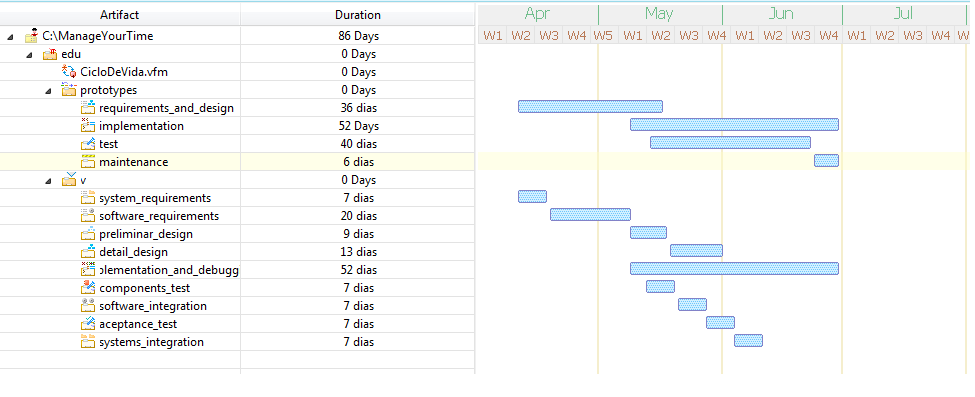
\includegraphics[width=0.7\linewidth]{proyecto/metodologia/imgs/Gantt}
	\caption{Cronograma. Diagrama de Gantt}
	\label{fig:gantt}
\end{figure}
\subsection{Metodología de implementación}
Los criterios que se establecieron al momento de justificar la elección los procesos de software prototipo y V, cuentan con la misma validez para determinar la metodología de implementación, debido a que para esta etapa también es necesario tener un plan de acción que beneficie la gestión de tiempos del proyecto, complemente los procesos de software, cumpliendo un proceder de forma organizada. Por esta razón se utilizará Scrum como metodología para implementar.
\begin{figure}
	\centering
	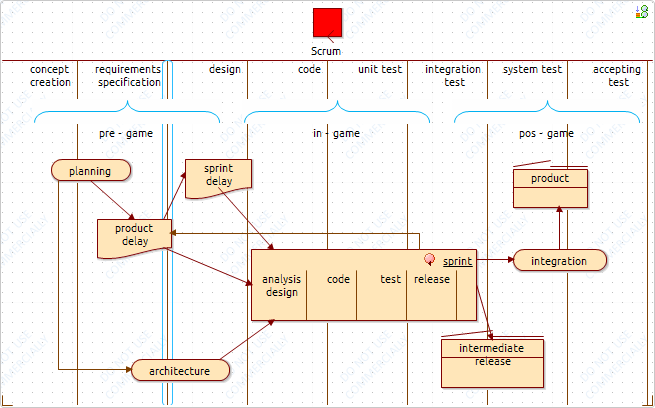
\includegraphics[width=0.7\linewidth]{proyecto/metodologia/imgs/Scrum}
	\caption{Scrum}
	\label{fig:gantt}
\end{figure}
\section{Open Source}
Desde que las personas empezaron a desarrollar software, han empezado a indagar en diferentes formas de realizar las cosas, a fin de obtener la solución computacional que solucione su necesidad. Con el tiempo estos pensamientos han devenido en ideologías que orientan la variedad de metodologías disponibles para desarrollar software.

El pensamiento o filosofía que entra en cuestión, es la del software libre, donde uno de sus principios, consiste en la reutilización del conocimiento, en este caso, el código. Es aquí donde entra el Open Source, que se relaciona con el código abierto, y con su revisión por parte de una comunidad de desarrolladores externos. Siguiendo el principio de filosofía libre, se pretende utilizar el concepto O.S con la intención de obtener una ayuda en momentos donde la implementación se torne complicada, llegandose a extrapolar a diversos casos en los que se necesite la apreciación del problema que se está trabajando por parte de un externo el cual ya lo haya desarrollado.
